\documentclass{IEEEtran}
\usepackage{amsmath}
\usepackage{amsfonts}
\usepackage{graphicx}
\usepackage{hyperref}
% \usepackage{cleverref}

\newcommand{\Gt}{\ensuremath{G_\text{true}}}
\newcommand{\Ct}{\ensuremath{C_\text{true}}}
\newcommand{\Nt}{\ensuremath{\mathcal{V}_\text{true}}}
\newcommand{\Et}{\ensuremath{\mathcal{E}_\text{true}}}
\newcommand{\Comt}{\ensuremath{\mathcal{C}_\text{true}}}

\newcommand{\Gs}{\ensuremath{G_\text{samp}}}
\newcommand{\Ns}{\ensuremath{\mathcal{V}_\text{samp}}}
\newcommand{\Es}{\ensuremath{\mathcal{E}_\text{samp}}}
\newcommand{\Coms}{\ensuremath{\mathcal{C}_\text{samp}}}

\newcommand{\target}{\ensuremath{\text{target}}}

\title{Activity Report: Targeted Network Discovery using a POMDP formulation}

\author{Zachary Sunberg\\Summer 2015}

\begin{document}
\maketitle

\begin{abstract}
This report gives a short overview of the investigation into a POMDP approach to a Social Network exploration problem conducted during the summer of 2015. I attempted to use a Monte Carlo Tree Search approach to solve the following problem online. Consider a social network with each member assigned to one of $M$ communities and edges between members generated according to a stochastic block model. Suppose that we are only given knowledge of a small subset of the edges and the community labels of a small subset of the vertices. We are also permitted to sequentially probe $T$ of the vertices, learning the neighbors of each probed vertex. The goal is to correctly guess the community label of a single target vertex given the network structure observed by probing.
\end{abstract}

\section{Background}

Exploration of social networks is a topic of active research. Many strategies have been proposed for sampling large graphs to accurately measure the properties of such graphs \cite{Leskovec2006, Seshadhri2014},
inferring community structure with incomplete information \cite{Caceres2014, Liu2015, Maiya2010, Yun2014},
learning about individuals based on features and network relationships \cite{Bilgic2010, Iii2012}, and selecting individual vertices to query to learn specific information about the graph \cite{Wang2013, Soundarajan2014}.

This work is most closely related to \cite{Soundarajan2014}. While these researchers attempted to identify graph characteristics such as the size of the largest connected component, vertex with the highest PageRank, and community structure based on a heuristic probing strategy, we attempt the less ambitious task of identifying the community affiliation of a single vertex. However, we adopt a principled approach modeling the problem as a Partially Observed Markov Decision Process (POMDP).

The POMDP framework is a system for modelling decision-making problems with uncertainty \cite{Kochenderfer2015}. In a POMDP, a policy determines an action to take based on incomplete knowledge of the true system state. This incomplete knowledge is known as the belief. A reward is received every time an action is taken, and the value of the reward is determined by the action and true system state. The policy seeks to maximize this reward by judiciously selecting actions.

The general problem of gathering information by probing a network is similar to a POMDP in that the true state (network structure) is unknown. However, it is difficult to state the problem as a POMDP in a strict sense because the goal of probing is to minimize the uncertainty in the belief, but the reward in a true POMDP is determined by the true state rather than the belief. Nevertheless, there has been some written about problems that have POMDP structure except that the reward is a function of the belief state rather than the true state. Such problems are known as $\rho$POMDPs \cite{Araya-Lopez2010}. The goal in such problems is to minimize the uncertainty (evaluated as the entropy for example) in the belief. Unfortunately, for network problems, the state of the network is usually too large for calculation of the exact belief after taking an action and receiving an observation to be computationally practical. For example, the set of all possible network structures for an undirected graph with $N$ vertices has a cardinality of $O\left(2^{N^2}\right)$ (each pair of vertices can either be connected or disconnected). Since the set of possible belief states is $[0,1]^{O\left(2^{N^2}\right)}$, even simply storage of the complete belief state is problematic.

Another way to evaluate the success of an exploratory probing policy is to have the policy make a guess at the answer to a question about the network after probing \cite{Mihaylova2003}. If the policy is usually able to answer this question correctly, then it is effective at exploring for the information in the question. For this research, the question answered by the policy after probing is ``\textbf{Which community does the target vertex belong to?}''. A potential real world example that this problem could represent is linking a terrorist to a terrorist organization.

Recent research explored the use of a Markov Decision Process (MDP) model for controlling the spread of infection on a network \cite{Ho2015}. Monte Carlo Tree Search (MCTS) was the most successful of the approaches used, so we used a variant of it on this problem. In the following sections, the problem formulation is given, followed by a description of the solution approach.


\section{Problem Description}

\begin{figure}[tb]
    \centering
    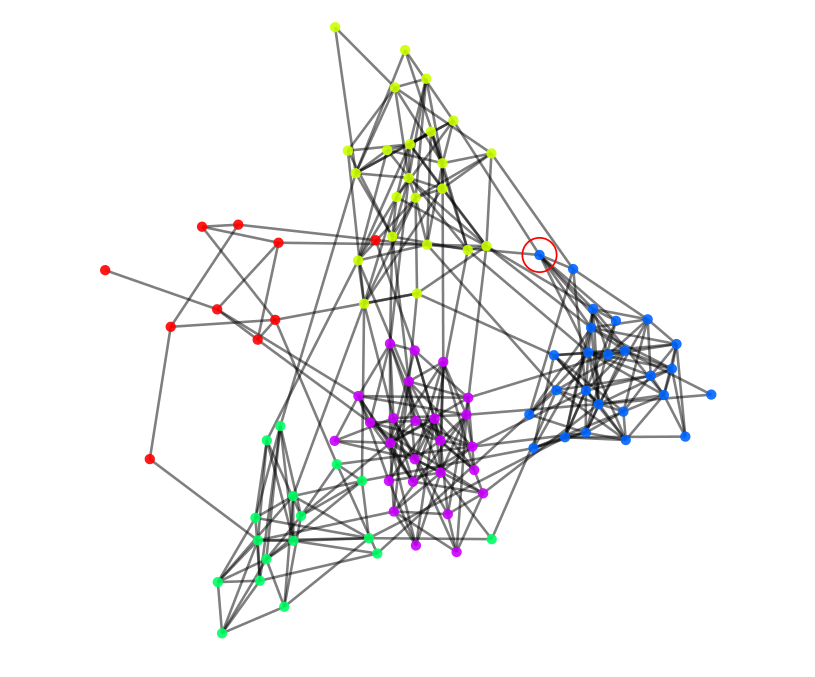
\includegraphics[width=\columnwidth]{network.png}
    \caption{An example social network. Community membership is indicated by the vertex's color. The target node is indicated by a red circle.}
    \label{fig:network}
\end{figure}

The objective is to efficiently explore a network by probing vertices to determine the network affiliation of a target vertex. The true network, $\Gt = (\Nt, \Et)$, is randomly generated and consists of $N=100$ vertices. Each vertex is assigned uniformly randomly to one of $M=5$ groups. This mapping from vertices to communities will be referred to as $\Comt : \Nt \to \{1\dots M\}$. Edges are generated according to a stochastic block model (SBM) \cite{Wang1987}, that is, two vertices within the same community are connected with a probability of $p_\text{inter} = 0.3$ and vertices not in the same community are connected with a probability of $p_\text{intra} =0.01$. An example network generated according to this method is shown in Figure~\ref{fig:network}.

The decision making agent is initially given partial information about the network. The graph $\Gs = (\Ns, \Es)$ is randomly sampled from $\Gt$ with $|\Ns| = N_0 = 10$ and $|\Es| = E_0 = 10$. Also a subset of $\Comt$, $\Coms$, is revealed, specifically the affiliations of all of the vertices in $\Ns$ are given. The agent also knows the number of vertices and communities in the network and statistical information used to generate the network, that is $p_\text{inter}$ and $p_\text{intra}$. In addition, the agent may choose $T$ vertices sequentially, and, after observing a vertex, gain full knowledge of all of the edges connected to that vertex.

After observing all $T$ vertices, the final action taken by the agent is to guess the answer to the question, and a reward is given if the answer is correct. This problem may be stated as a POMDP. A POMDP is defined by the tuple ($S$, $A$, $T$, $R$, $O$, $Z$):

\begin{itemize}
    \item The \textbf{state space}, $S$, is the set of all possible social networks involving the $N$ members of the network and their community affiliations. The true state is the true social network and community mapping, that is $s = (\Gt, \Comt)$.
    \item The \textbf{action space}, $A$, is the set of all possible actions at each step of the simulation. For each time step in $1..T$, the action is the choice of which vertex to query from the list of known vertices. At time $T+1$, the action is a guess of the community label of the target vertex.
    \item The \textbf{transition probability distribution}, $T:S \times A \times S \to [0,1]$ encodes how the state changes by specifying the probability of state $s$ transitioning to $s'$ given action $a$. In this problem, the state remains constant, so the probability distribution is simply an indicator function, $T(s, a, s') = \mathbf{1}(s = s')$. However, it would be reasonable for the social network to change slowly over time. This can be easily modeled in the POMDP framework and should be investigated in the future.
    \item The \textbf{reward function}, $R: S \times A \to \mathbb{R}$ returns the reward gained by executing action $a$ in state $s$. Since the only reward is given for guessing the correct community affiliation of the target vertex at the end of the problem, it is defined as
        \begin{equation}
            R(s_t, a_t) = 
            \begin{cases}
                100\cdot \mathbf{1}(a_t = \Comt(\target)) & \text{ if } t = T+1 \\
                0 & \text{otherwise}
            \end{cases}
        \end{equation}
        In future problem formulations, there may also be costs associated with measuring particular vertices.
    \item The \textbf{observation space}, $O$, is the set of all possible observations that could be produced after taking action $a$ in state $s$. At each time step, the observation is the set of neighbors of the vertex probed as specified by the action.
    \item The \textbf{observation distribution}, $Z:A \times S \times O \to [0,1]$ yields the probability of observation $o$ given that action $a$ was taken and the resulting state is $s'$. Since the observations are deterministic, this is an indicator function, $Z(a, s', o) = \mathbf{1}(o = \text{neighbors}_{s'}(a))$. Noisy measurements could be incorporated into the model easily by spreading out this distribution.
\end{itemize}

The objective of a POMDP is to find an optimized policy, $\pi^*$, that will specify an action given the initial information about the problem and the sequence of actions and observations received up to the current time. Let $I_t$ be the information vector at time $t$, that is, the information known about the network at the beginning of the problem, and the sequence of actions and observations up to time $t$,

\begin{equation}
    I_t = (\Gs, \Coms, a_0, o_1, a_1, \dots a_{t-1}, o_t) \text{.}
\end{equation}

The optimization objective is

\begin{equation*}
\begin{aligned}
& \underset{\pi}{\text{maximize}}
& & R \left( s_{T+1}, \pi(I_{T}) \right) \\
& \text{subject to}
& & I_{t+1} = (I_t, \pi(I_t), o_t), \quad t = 0 \dots T-1 \\
& & & I_0 = (\Gs, \Coms)
\end{aligned}
\end{equation*}

\section{Solution Approach}

In order to evaluate the effectiveness of using a POMDP approach for this problem, we compare it to a simple heuristic which will be described first, followed by the description of the POMDP solver. 

\subsection{Heuristic} \label{sec:heuristic}

The heuristic approach selects vertices to probe without considering the future consequences, that is, it is a myopic policy. It simply probes the vertices with the highest observed degree, a strategy that was reported to be successful for different tasks in \cite{Soundarajan2014}. This is not a particularly good approach for the task at hand; it would likely be easy to specify a much better heuristic. However it serves as a baseline with which to compare strategies.

Specifically, at steps 1 through $T$, this heuristic policy considers all of the vertices and edges that have been revealed and chooses to probe the unprobed vertex with the highest revealed degree, that is, the largest number of revealed incident edges. At step $T+1$, the policy must make a guess of the target vertex's affilitation. To do this, it first considers each neighbor, $n$, of the target vertex. If $n$ is unlabeled, the policy labels it with the label that is most common in the neighbors of $n$, breaking ties randomly. If $n$ has no labeled neighbors, it is left unlabeled. Once all neighbors of the target are labeled, the target label is guessed to be the most common label among the target neighbors with ties again broken randomly.

\subsection{Monte Carlo Tree Search}

The POMDP solution approach is Monte Carlo Tree Search (MCTS) \cite{Browne2012} on the belief state space. This is an online approach, that is, it carries out the computations to determine the best action at time $t$ \emph{after} all of the observations up to time $t$ have been received instead of calculating the best response to all potential observations beforehand (an offline solution). In order to do this, the algorithm uses Monte Carlo simulations to construct a tree with alternating layers of nodes corresponding to actions and observations. Each observation node corresponds to a belief, and each action node has a corresponding value estimate, $V_a$. This value estimate represents the expected reward accumulated by taking the action and following the optimal policy in the future. At each iteration, a new set of action nodes is added to the tree. Rollout simulations using a heuristic rollout policy provide unbiased estimates of the value. Details of the algorithm can be found in the journal article describing the POMCP algorithm \cite{Silver2010}, though this algorithm is not strictly POMCP because it does not use the particle filter belief updates described in the paper.

The expansion of the tree is carried out in an optimistic manner, i.e. the actions that yield higher rewards are explored more thoroughly. However, if the action with with the highest value were chosen to be explored every time, the algorithm would not perform well because of under-exploration. In order to mitigate this problem, the ``Upper Confidence Bound for Trees'' (UCT) modification is used \cite{Browne2012}. In this approach, the algorithm explores the action that has the highest score according to
\begin{equation}
    V_a + c \sqrt{\frac{\log{(N_o)}}{N_a}} \text{,}
\end{equation}
where $c$ is an adjustable parameter controlling the greediness of the exploration, $N_o$ is the number of times that the parent observation node of the action node has been observed, and $N_a$ is the number of times that the action node has been chosen.

Typically, instead of using the action-observation history, $I$, directly as feedback, the policy makes its decision based on a belief representation, $b$, that is a probability distribution over $S$ that is a sufficient statistic for the action-observation history (that is, it contains the same information as the history) \cite{Kochenderfer2015}. As mentioned before, an exact belief distribution over all possible graph structures is much too large to be practical. Because of this, we use a belief representation that consists of a list of all the edges and vertices observed in the initial sample and the subsequent probes.

In order to run the Monte Carlo simulations, this belief is ``sampled'' by generating a complete network (state) in the following manner. First the edges in the original sample, $\Es$, and the edges observed by probing are added to the sampled network. Next, the community affiliation of the vertices \emph{that are neighbors of the known community nodes in $\Coms$} is inferred using $p_\text{intra}$, $p_\text{inter}$, and Bayes rule. The community affiliations of the remaining vertices are assigned randomly, and the remaining edges are generated according to the stochastic block model with $p_\text{intra}$ and $p_\text{inter}$.

When simulations are continued beyond the depth of the tree, a rollout policy must be used to determine the actions for the simulation. The rollout policy used in our work is the highest degree heuristic described in Section~\ref{sec:heuristic}.

\section{Results}

In a set of 100000 tests, the heuristic was able to guess the correct target vertex affiliation about $41\%$ of the time (random guesssing would result in a $20\%$ success rate.

Small mistakes in the problem implementation were repeatedly discovered, so unfortunately none of the results produced by the MCTS solver can be reported with confidence in their correctness. At the end of the research period, the MCTS solver was not scoring better than the expected score for random guessing (20).

A visualization of the tree that MCTS constructed for one of the problems is shown in Figure~\ref{fig:tree}. This visualization was captured after only a small number (30) tree exploration iterations, so it is much smaller than the trees actually used for decision making.

\begin{figure}[tb]
    \centering
    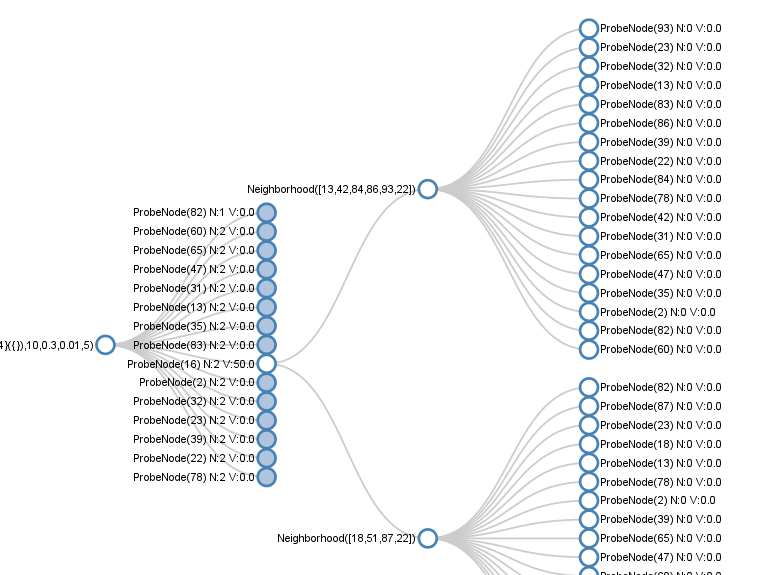
\includegraphics[width=\columnwidth]{POMCPTree.png}
    \caption{Example MCTS Tree after 30 iterations. The node on the left is the root node. The first column of nodes correspond to actions. All of these nodes have been explored (N>0 for all of them), but their subtrees are not shown for clarities sake. The displayed subtree shows the next level of observation nodes and action nodes.}
    \label{fig:tree}
\end{figure}

The code used for this project is available at \url{https://github.com/sisl/NetworkDiscovery.jl}.

\section{Future Work}

There are a variety of directions for this work to be carried into. The first task would be deeper investigation into why MCTS is not working correctly for the current problem. The heuristic could also be improved and tailored more specifically to this problem for better performance. For example, a heuristic that queries the neighbors of the target node would probably work very well. The problem could also be made more difficult within the current framework by allowing the network to change slowly over time or producing noisy observations. Finally the POMDP approach may be extended to other problems, for example the goal could be to probe nodes for the purpose of guessing the labels of as many nodes as possible.

\bibliographystyle{unsrt}
\bibliography{Network_Discovery.bib}

\end{document}
